\RequirePackage[orthodox]{nag}
\documentclass[11pt]{article}

%% Define the include path
\makeatletter
\providecommand*{\input@path}{}
\g@addto@macro\input@path{{include/}{../../include/}}
\makeatother

\usepackage{../../include/akazachk}

\title{Systems Identification - 111106}
\author{Andres Espinosa}
\begin{document}
\pgfplotsset{compat=1.18}
\maketitle

\tableofcontents

\section{Introduction}
\subsection{Concepts}
This course will explore a few broad topics listed below
\begin{itemize}
    \item Systems Identification
    \item State Estimation
\end{itemize}
The first section of the class will start with systems identification, we will then go over state estimation at the end.

\subsection{What is Systems Identification?}
Identifying a system deals with building a model with the goal of representation a system.
State equations, transfer functions, and frequency/step responses are mathematical ways that we can describe a system.
Graphical representations can also be useful to identify a system in a visual way.
Often, depending on the system, a photo or diagram of a system can be a useful way to extract information and gather insights.
We can also have code representations which attempt to model system logic through programmatic rules.
Physical models exist such as that of a scale representation attempts to simulate a system through simplification and minimizing the scale model of the actual system.

A dynamic system is a system that varies over time and doesn't just have an input and output but evolves over time.
On the other hand, a static system is a system that is only dependent on a transformation from its inputs to its outputs.
By building models, we can attempt to represent these systems in a few ways.
Continuous time models attempt to divide time into the true continuous time stream, where discrete times bucket time into discrete intervals.
There are also linear and nonlinear models that are used to represent systems, sometimes regardless of their linearity.

\begin{figure}[h]
\centering
\begin{tikzpicture}[>=latex, thick, node distance=2.4cm]
% Static system
\node (u_s) {$u(t)$};
\node[draw, rectangle, minimum width=1.8cm, minimum height=1.0cm, right=1.2cm of u_s] (S) {$f(\cdot)$};
\draw[->] (u_s) -- (S);
\node[right=1.2cm of S] (y_s) {$y(t)$};
\draw[->] (S) -- (y_s);
\node[below=0.25cm of S] {Static: $y(t)=f\!\big(u(t)\big)$};

% Dynamic system
\node[right=4.4cm of y_s] (u_d) {$u(t)$};
\node[draw, rectangle, minimum width=2.2cm, minimum height=1.0cm, right=1.2cm of u_d] (D) {$G$};
\draw[->] (u_d) -- (D);
\node[right=1.2cm of D] (y_d) {$y(t)$};
\draw[->] (D) -- (y_d);

% State feedback loop (memory)
\node[draw, circle, minimum size=6mm, above=1.0cm of D] (x) {$x$};
\draw[->] (x) -- (D);
\draw[->] (D) |- +(0,1.05) -| (x);

\node[below=0.25cm of D, align=center] {Dynamic: $\dot x(t)=g\!\big(x(t),u(t)\big)$\\$y(t)=h\!\big(x(t),u(t)\big)$};
\end{tikzpicture}
\caption{Static system: output depends only on present input. Dynamic system: output depends on present input and an internal state that evolves over time.}
\end{figure}

\subsection{Why Create Models?}
After creating model representations of systems, we can use the model for various reasons.
One of which is simulation. 
After creating a model, we can use a simulation to approximate and identify how a system would behave under different parameters without spending the real life physical cost associated with doing so.
We can also use a model to tune individual parameters that we have control over in the system and better design our system.
Models can also be used to design controls and vary our input parameters better.
\begin{itemize}
    \item Simulation
    \item Parameter Tuning (System Design)
    \item Controls
    \item State Estimation
    \item Fault Detection
    \item Prediction
\end{itemize}

\subsection{Models}
Different properties exist that divide models into distinct categories that inform their development and characteristics.
\begin{itemize}
    \item Discrete-time vs Continuous: Discrete timesteps $k \in \mathbb{Z}$ vs a continuous time frame $t \in \mathbb{R}$.
    \item Time-varying vs Invariant: A time-varying model has properties that change over time where as a time-invariant model does not evolve or change over time.
    \item Parametric vs Non-Parametric: A parametric model has a finite number of parameters that can be linear or non-linear.
    \item Linear vs Non-Linear: Most systems are non-linear but we can use linear models to approximate or non-linear models to attempt to model a higher degree of complexity.
\end{itemize}

\subsection{Linear Models}

\subsubsection{Box Car Example}

The system depicted in Figure \ref{fig:box_car} is a linear time-invariant system.
The spring acts with $Kp$ and the dampener counteracts it with $Cv$
\begin{equation}
    Ma = F - Kp - Cv
\end{equation}
By changing this equation where $F = u(t)$ is our input which represents our input force  and $p = y(t)$ is our output which represents the position of the car.
\begin{equation}
    M y^{\prime \prime} + C y^\prime + K y = u 
\end{equation}

\begin{figure}[h]
\centering
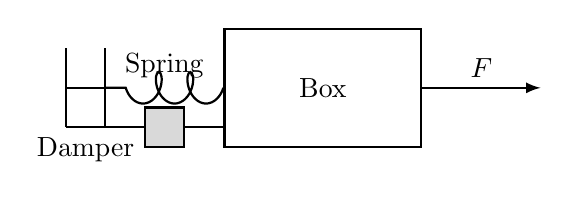
\begin{tikzpicture}[>=latex, thick, node distance=1.5cm]
% Car
\node[draw, rectangle, minimum width=2.5cm, minimum height=1.5cm] (car) {Box};

% Spring
\draw[decorate, decoration={coil, aspect=0.6, segment length=4mm, amplitude=2mm}] 
    (car.west) -- ++(-1.5cm, 0) node[midway, above] {Spring};

% Damper (parallel to spring)
\draw[thick] (car.west) ++(-1.5cm, -0.5cm) -- ++(-0.5cm, 0) 
    node[midway, below] {Damper};
\draw[thick] (car.west) ++(-1.5cm, -0.5cm) -- ++(0, 1cm);
\draw[thick] (car.west) ++(-2cm, -0.5cm) -- ++(0, 1cm);
\draw[thick] (car.west) ++(-2cm, 0) -- ++(0.5cm, 0) 
    node[midway, above] {};

\draw[thick] (car.west) ++(-2cm, -0.5cm) -- ++(2cm, 0cm);
\draw[thick, fill=gray!30] (car.west) ++(-1cm, -0.75cm) rectangle ++(0.5cm, 0.5cm);

% Force
\draw[->] (car.east) -- ++(1.5cm, 0) node[midway, above] {$F$};
\end{tikzpicture}
\caption{Box car diagram with a spring and a parallel damper on the left, and a pulling force on the right.}
\label{fig:box_car}
\end{figure}

A linear system has this equation $y(t) = y_f(t) + y_0 (t) $.
There are two special scenarios for a linear system:
One where the initial conditions are zero and we force an input to directly map to the output (forced output $y_f$),
and one where no input is ever forced into the system but the initial condition is not zero (free output $f_0$).

A property of linear systems is that, in the context of a forced output, any input can be represented as a linear combination of other inputs and the output will be the same linear combination of the corresponding outputs.

More simply, consider $x(0) = 0$ (initial state/conditions is null/zero), the following is a property of linear systems.

For a $u_1(t) \rightarrow y_1(t)$ and $u_2(t) \rightarrow y_2(t)$ and two scalars $\alpha, \beta$

\begin{equation}
    u(t) = \alpha u_1(t) + \beta u_2(t) \implies y_f(t) = \alpha y_1(t) + \beta y_2(t)
\end{equation}

\subsubsection{System Vs Model}
In the example in Figure \ref{fig:box_car}, it is easy to see that this model isn't a perfect representation of the actual system.
Friction is an important component that would introduce complexity and non-linearity.
$S = M(\theta)$ or $S=M$ means that for the purpose of the math exercise, the system is perfectly represented by its model and its parameters.

\subsubsection{Circuit Model - Nonlinear}
As an example, we can have a small system that is a battery - resistor - capacitor - ground circuit in series.

\begin{figure}[h]
\centering
\begin{circuitikz}[american]
    % Battery
    \draw (0,0) to[battery, l=$V_b(t)$] (0,2)
              to[short] (2,2)
              to[R, l=$R$] (4,2)
              to[short] (4,1)
              to[C, l=$C$] (4,-1)
              to[short] (2,-1)
              to[short] (0,-1)
              to[short] (0,0);
    % Label for capacitor voltage
    \node at (4.5, 0) {$V_c(t)$};
\end{circuitikz}
\caption{Battery-resistor-capacitor circuit in series.}
\label{fig:circuit_model}
\end{figure}

\begin{equation}
    V_b(t) = R i(t) + V_c (t)
\end{equation}
This equation can be turned into a model by having the input be the battery voltage inputted and the output be the voltage of the capacitor.
\begin{equation}
    u(t) = y(t) + RC y^\prime(t)
\end{equation}

This isn't a linear system since there will be a breaking point that will explode the capacitor if overfilled with voltage.
Although our linear model is an approximation for this more complex system, this can generally be enough for a lot of applications.
The system will frequently be "linear enough" when values are reasonably constrained or small.

\subsection{September 30th}
A transform function takes a space that it in a different domain (like time) and turns it into another domain (like complex space).
\begin{equation}
    Y_f(s) = T(s) U(s)
\end{equation}

The transfer function works with the forced output, not the free output. 
Another way to describe a transfer function is the laplace transform of the forced impulse response.
\begin{equation}
    T(s) = L \{ h(t) \}
\end{equation}

\begin{equation}
    y_f(t) = h(t) \ast u(t) = \int_{0}^{\tau} h(\tau) u(t-\tau) d \tau
\end{equation}

A system can be split into its controllable and observable parts.
A transfer function $T(s)$ works with the inputs that are both controllable and observable.
A frequency response $T(jw)$ is a transfer function that is computed in imaginary component.

\subsubsection{Plant Example}
Consider an asymptotically (it will become stable over time with any initial conditions and no input) stable plant with transfer function $G(s)$
\begin{equation}
    u(t) = \sin (wt)
\end{equation}

Since the system is asymptotically stable, after some time the free output will converge to zero and the forced output will converge to an amplified sinusoid similar to the input sinusoid.
\begin{equation}
    y_f (t) = |G(j \omega)| \sin (\omega t + \angle G(jw))
\end{equation}
where $|G(j \omega)|$ is the radius $r$ and $\angle G(jw)$ is the angle $\theta$ that the point makes with the real and imaginary plane.

\subsection{October 6th}

\subsubsection{Systems ID Types}
Black box methods of systems identification represent attempting to identify the system without information on the system's dynamics or parameters.
In order to attempt to solve it, we feed in inputs $u(t)$ and record the outputs $y(t)$ to create a dataset $D=((u_1, y_2), \dots)$.
We can identify a possible type of function, for example a rational transfer function 
\begin{equation}
    G(s) = \frac{b_m s^m + \dots + b_1 s + b_0}{a_n s^n + \dots + a_1 s + a_0}
\end{equation}

and use our dataset to attempt to fit the parameters ($a,b$) and meta-parameters ($n,m$) to the problem.

We also have a grey-box approach in which we have a known structure but we do not know the specific parameters to the system.
For example, a physics system in which we know the components in play but we do not know exact specifications like the mass or different physics constants.
We can similarly conduct experiments to attempt to parameterize the system.

Ad-hoc methods or tailor-made methods are very specific methods used to identify systems in specific domains.

\subsubsection{Frequency vs Step Response}



\section{EXTRA: Systems and Signals}
\subsection{Background}
\subsubsection{Complex Numbers}
Electrical engineers use the notation $j$ instead of $i$ for complex numbers.

\begin{equation}
    j^2 = -1 \quad \text{and} \quad \sqrt{-1} = \pm j
\end{equation}

\end{document}